% thesis using usydthesis.cls - Andrew Mathas 5/2002
\documentclass[BSc]{usydthesis}
% \includeonly{chapt1}
%%%%%%%%%%%%%%%%%%%%%%%%%%%%%%%%%%%%%%%%%%%%%%%%%%%%%%%%

\author{Ragib Zaman}
\title{Optimization of Bregman Divergences}

%%%%%%%%%%%%%%%%%%%%%%%%%%%%%%%%%%%%%%%%%%%%%%%%%%%%%%%%

% causes equations to be numbered as section.equation
\numberwithin{equation}{chapter}

\theoremstyle{remark}

\newtheorem{Definition}[equation]{Definition}
\newtheorem{Theorem}[equation]{Theorem}
\newtheorem{Proposition}[equation]{Proposition}
\newtheorem{Lemma}[equation]{Lemma}
\newtheorem{Corollary}[equation]{Corollary}

\newtheorem{Remark}[equation]{Remark}
\newtheorem{Example}[equation]{Example}

%%%%%%%%%%%%%%%%%%%%%%%%%%%%%%%%%%%%%%%%%%%%%%%%%%%%%%%%

% personal macros

% natural numbers, real numbers, etc
\newcommand{\N}{\mathbb{N}}
\newcommand{\R}{\mathbb{R}}
\newcommand{\C}{\mathbb{C}}
\newcommand{\Z}{\mathbb{Z}}
\newcommand{\Proj}{\mathbb{P}}
\newcommand{\T}{\mathbf{\theta}}
\newcommand{\face}{\prec}
\newcommand{\V}{\vee}
\newcommand{\la}{\lambda}

\newcommand{\Lag}{\mathcal{L}}
\newcommand{\M}{\mathbf{\mu}}
\newcommand{\E}{\mathbb{E}}
\newcommand{\x}{\mathbf{x}}
% macros for End(X) and Hom(X,Y)
\DeclareMathOperator{\End}{End}
\DeclareMathOperator{\Hom}{Hom}
\DeclareMathOperator{\im}{im}
\DeclareMathOperator{\Cone}{Cone}
\DeclareMathOperator{\Spec}{Spec}
% for f:X -> Y; the default spacing isn't great
\newcommand{\map}[2]{\,{:}\,#1\!\longrightarrow\!#2}
\newcommand{\B}[1]{\mathbf{#1}}
% example \varphi \map{X}{Y}

%Short Exact Sequences e.g \ses{X}{f}{Y}{g}{Z} will produce the s.e.s 0 to X to Y via f to Z via g to 0

\newcommand{\ses}[5]{
  \begin{equation*}
    0\xrightarrow{}
    #1\xrightarrow{#2}
    #3\xrightarrow{#4}
    #5\xrightarrow{}
    0
  \end{equation*}
}
%%%%%%%%%%%%%%%%%%%%%%%%%%%%%%%%%%%%%%%%%%%%%%%%%%%%%%%%

%In the intro remark where we could have been more general (k instead of C, ...

\begin{document}  

% roman page numbers for the initial pages
\pagenumbering{roman}

\maketitle          % creates the title page
\chapter*{Abstract}
In this report we survey Bregman Divergences and motivate their study by forming connections to areas such as convex optimization, machine learning and statistics. We give particular focus to developing an understanding of the optimization of Bregman Divergences and the connection to Exponential Families and Logistic Regression. In the second chapter we see that the Kullback-Liebler divergence between two members of an exponential family can be expressed as a Bregman Divergence between the distribution parameters. The third chapter gives a brief overview of Generalized Linear Models and Logistic Regression. We give a moderately simplified proof of a theorem of A.~ Banerjee (\cite{logodds}) which states that the log-odds ratio of the class posteriors is affine (which is the modelling assumption of Logistic Regression) if and only if the class conditional distributions belong to a fixed natural exponential family. In the final chapter, we show how the problem of finding the optimal parameters for the log loss of Logistic Regression can be cast as a Bregman Divergence optimization problem, and prove the convergence of an algorithm for finding those parameters using methods standard in the optimization of Bregman divergences. By simplifying their assumptions and/or proofs where we were able to, we believe we have given a clearer presentation of the results which we have drawn from our references. We hope that the reader will come away with a keen interest in Bregman Divergences and be aware of potential applications in their fields of study.\\ 
\section*{Acknowledgments}
First and foremost I would like to thank Dr. Cheng Soon Ong. I greatly value the wisdom he has shared with me, helping me identify the core ideas in machine learning and the links between. His willingness to give his time so generously and with such patience has been very much appreciated.\\

I would also like to thank Dr. Weifa Liang and Dr. Stephen Gould for taking the responsibilities of course convener and examiner respectively. Without their contribution I would not have been able to have the pleasure of completing this course. 
\tableofcontents    % creates the table of contents

% reset the page numbering and change to arabic numbers
\newpage\setcounter{page}{1}\pagenumbering{arabic}

\chapter{Bregman Divergences}
\section{Introduction}
The notion of convexity and the properties of convex functions have proven to be very useful, fundamentally due to them being the largest class of function for which we can develop a satisfactory theory of optimization for. As such, convex functions appear naturally as objects of interest in any field which utilizes optimization, such as machine learning, statistics, control theory, quantitative finance and many more. \\

Bregman divergences encode more precise information about convexity. Suppose that $\Delta\subseteq \mathbb{R}^m$ is a convex set and $F \map{\Delta}{\mathbb{R}}$ is continuously differentiable. Then $F$ is a convex function if and only if $ F(p) - F(q) - \langle \nabla F(q), p-q \rangle \geq 0$ for all $p,q \in \Delta.$ This leads to the definition of Bregman Divergences.

\begin{Definition}
 Let $F: \Delta \to \mathbb{R}$ be a strictly convex function, continuously differentiable on a closed convex set $\Delta\subseteq \mathbb{R}^m.$ The {\em Bregman Divergence generated by $F$} is the function $B_F : \Delta \times \Delta \to \mathbb{R}$ defined by $$ B_F(p,q) = F(p) - F(q) - \langle \nabla F(q), p-q \rangle$$ 
\end{Definition}

We have restricted the generators of Bregman Divergences to be strictly convex functions so as to be consistent with most other sources. This restriction allows Bregman Divergences to satisfy certain additional properties which we will soon discuss. It is important to note however that some of the properties we discuss do not require the convexity of $F,$ and interesting results can be obtained by considering Bregman Divergences generated by more general $F$ (for example, see \cite{Cheng}).  


\begin{Example} Two familiar examples are:
 \begin{itemize}
 \item Squared Mahalanobis Distance
 \\
 Let $F:\mathbb{R}^m \to \mathbb{R}, x \mapsto x^TQx,$ where $Q$ is a positive definite matrix. Then $B_F(p,q) = (p-q)^T Q (p-q).$ When $Q = I_m,$ this is the squared Euclidean distance.
 
 \item Kullback-Leibler Divergence (also known as Relative Entropy) 
 \\
 Let $F:(\mathbb{R}_{>0})^m \to \mathbb{R}, x \mapsto \sum_{i=1}^m x_i \log x_i.$ Then $$B_F(p,q) = \sum_{i=1}^m  \left( p_i \log\left(\frac{p_i}{q_i}\right) -p_i + q_i\right)$$ 
\end{itemize}
\end{Example}
\section{Properties}
\begin{Proposition}{The following statements are true for Bregman Divergences:}\\
 \begin{itemize}
  \item Positive Definiteness: $B_F(p,q)\geq 0$ for all $p,q,$ with equality if and only if $p=q.$
  \item Convexity: $B_F(p,q)$ is convex in its first argument.
  \item Conic Property: For $\alpha, \beta>0$ we have $B_{\alpha F_1 + \beta F_2}(p,q) = \alpha B_{F_1}(p,q) + \beta B_{F_2}(p,q).$
  \item Gradient in first argument: $\nabla_p B_F(p,q) = \nabla F(p) - \nabla F(q).$
  
 \end{itemize}

\end{Proposition}

\begin{proof}
 The Non-negativity of $B_F$ is precisely the 1st order characterization of the convexity of $F.$ The convexity of $B_F$ in the first argument follows from the convexity of $F.$ The Conic property follows immediately from the definition. If we allowed non-convex generators then we would not require the condition $\alpha, \beta>0,$ and this property would instead be linearity. Many authors refer to this property as linearity anyway, despite requiring strictly convex generators. The Gradient follows easily from the definition.
\end{proof}

Given a strictly convex function $F,$ a naturally related strictly convex function is its convex conjugate (or Legendre-Fenchel transform). It turns out that the Bregman Divergences which they generate are closely related as well. First we recall a property of conjugates.

\begin{Lemma}\label{invert}
 Let $F^*(q) = \sup_{p\in \Delta} ( \langle p, q \rangle - F(p) )$ denote the convex conjugate of $F$ which is strictly convex and continuously differentiable. Then for all $p\in \Delta,$ we have
 
 $$(\nabla F^*)(\nabla F(p)) = p$$
 so $\nabla F$ is an invertible function from $\Delta$ onto its range, with its inverse being $\nabla F^*.$ Also, $\operatorname{dom}(F^*)$ is the range of $\nabla F.$
\end{Lemma} 
 \begin{proof}
  Take a fixed $p\in \Delta.$ By the first order condition, $p$ is the maximizer in the definition $F^*(q) = \sup_{p\in\Delta} ( \langle p,q\rangle - F(p)),$ if and only if $q = \nabla F(p)$ (otherwise the supremum is infinite, so $\operatorname{dom}(F^*)$ is the range of $\nabla F$). We have $F^*(q) + F(p) = \langle p,q\rangle.$ Since $F$ is continuous and strictly convex, we have $F = F^{**}$ by the Biconjugation theorem (\cite{Bi}). Thus, we have 
\begin{equation}
F^*(q) + F^{**}(p) = \langle p,q\rangle \label{q}
\end{equation}
 implying that $q$ is the maximizer in $F^{**}(p) = \sup_{r\in\Delta} ( \langle p, r \rangle - F^*(r)).$ The first order condition then implies that $p = \nabla F^*(q) = \nabla F^*( \nabla F(p)).$ 
 \end{proof}


\begin{Theorem}
 Let $F$ be strictly convex and continuously differentiable. Then for all $p\in \Delta, q\in \operatorname{dom}(F^*),$ we have
 $$ B_{F^*}(\nabla F(q), \nabla F(p)) = B_F(p,q).$$
\end{Theorem}

\begin{proof}

 By \eqref{q} we have $F^*( \nabla F(p)) = \langle p, \nabla F(p)\rangle - F(p),$ which lets us compute
 
 \begin{align*}
  B_{F^*} ( \nabla F(q), \nabla F(p)) &= F^*(\nabla F(q)) - F^*(\nabla F(p)) - \langle \nabla F^*( \nabla F(p)), \nabla F(q) - \nabla F(p)\rangle \\
  &= \langle q, \nabla F(q)\rangle - F(q) - \langle p, \nabla F(p)\rangle + F(p) - \langle p, \nabla F(q) - \nabla F(p)\rangle \\
  &= F(p) - F(q) - \langle \nabla F(q), p-q\rangle\\
  &= B_F(p,q).
 \end{align*}


\end{proof}

The results and examples seen above indicate that Bregman Divergences seem to capture some notion of distance. While they do not define metrics, they sometimes behave like a 'squared metric'. We now prove an important result that connects whatever notion of distance Bregman Divergences capture to means.

\begin{Theorem} (Mean is the Minimizer)\\
 Suppose $P$ is any random variable taking values in $\Delta$ with distribution $\mathcal{D}.$ Then $q \mapsto \mathbb{E}_{P \sim \mathcal{D}}[ B_F(P,q)]$ is minimized uniquely at $q^* = \mathbb{E}_{\mathcal{D}}[P].$ Note that this minimizer is independent of $F.$
\end{Theorem}

\begin{proof}
 Let $q$ be any fixed point in $\Delta.$ Applying the definitions and linearity of expectation, we have 
 
 \begin{align*}
  \mathbb{E}[ B_F(P,q)] - \E[B_F(P,q^*)] &= \E[ F(P)-F(q) - \langle \nabla F(q), P-q \rangle - F(P) + F(q^*) + \langle \nabla F(q^*), P-q^* \rangle ] \\
  &= F(q^*) - F(q) + \langle \nabla F(q), q \rangle - \langle \nabla F(q^*), q^* \rangle \\
  & \ \ + \E[\langle \nabla F(q^*), P \rangle - \langle \nabla F(q), P \rangle] \\
  &= F(q^*) - F(q) + \langle \nabla F(q), q \rangle - \langle \nabla F(q^*), q^* \rangle \\
  & \ \ + \langle \nabla F(q^*)-\nabla F(q), \E[P] \rangle \\
  &= F(q^*) - F(q) - \langle \nabla F(q), q^* - q \rangle \\
  &= B_F(q^*, q)
 \end{align*}
Since $B_F(q^*,q)\geq 0$ with equality if and only if $q=q^*,$ we have the result.
\end{proof}

The following converse result also holds. 
 \begin{Theorem}(Banerjee et al, 2005, \cite{mean})\\
  Suppose $\Delta\subseteq \mathbb{R}^m $ is a closed convex set and $d: \Delta \times \Delta \to \mathbb{R}$ is a continuously differentiable positive definite function. If $q=\mathbb{E}[P]$ is the unique minimizer of $\mathbb{E}[d(P,q)]$ for all random variables $P$ taking values in $\Delta,$ there exists a strictly convex differentiable function $F:\Delta\to\mathbb{R}$ such that $d = B_F.$
 \end{Theorem}
\newpage
\section{Optimization}

We have seen that Bregman Divergences convey a notion of distance and that they are convex functions in their first argument. Thus, a natural optimization problem that often arises is to find the {\em Bregman projection} of a vector $q_0 \in \Delta \subseteq \mathbb{R}^m$ onto a linear subspace. Suppose we wish to find the $p\in \Delta$ which has least Bregman divergence to $q_0$ and satisfies some linear equality constraints. We explore a specific case below. \
\newline \\

$\mathbf{Problem}-$
Suppose $F$ is continuously differentiable. Further assume that the domain of $F^*$ is $\mathbb{R}^m,$ which by Lemma \ref{invert}  is equivalent to $\nabla F : \Delta \to \mathbb{R}^m$ being a bijection. Let $\mathcal{P} = \{ p \in \Delta \ | \ p^TM = \tilde{p}^TM\}$ be the set of points satisfying the constraints, where $M$ is some $m\times n$ matrix and $\tilde{p}\in \Delta.$ Note $\tilde{p}\in\mathcal{P}$ so $\mathcal{P}$ is non-empty. We wish to find $q_*=\arg \min_{p\in \mathcal{P}} B_F(p, q_0).$\
\newline \\
Towards solving the problem, let us define the {\em Legendre-Bregman projection} $\Lag : \Delta \times \mathbb{R}^m \to \Delta$ as
$$ \Lag_F(q,v) = (\nabla F)^{-1} ( \nabla F (q) - v),$$
which is well defined under our assumptions on $F.$ Let $\mathcal{Q} := \{ \mathcal{L}_F(q_0, M\lambda) \ | \lambda \in \mathbb{R}^n \} \subseteq \Delta.$ Note $q_0\in\mathcal{Q}$ so $\mathcal{Q}$ is non-empty.\
\newline \\
The Lagrangian of our problem is given by $$K(p,\lambda) = B_F(p,q_0) + (p^TM - \tilde{p}^TM)\lambda.$$

By the theory of Lagrange multipliers, the solution to the problem is given by the saddle point of the Lagrangian, where the minimum is taken with respect to $p$ and the maximum with respect to $\la.$ To minimize with respect to $p$ we require
$\nabla_p K(p,\lambda) = 0$ which we can write as  $$\nabla F(p) = \nabla F(q_0) - M\lambda.$$ Applying $(\nabla F)^{-1}$ to both sides yields $p = \mathcal{L}_F(q_0, M\lambda)\in \mathcal{Q}.$ To maximize with respect to $\la,$ we require $\nabla_{\lambda} K(p,\lambda)= 0,$ which is simply the condition  $p \in \mathcal{P}.$ Therefore, solving the problem is equivalent to finding a point in $\mathcal{P}\cap \mathcal{Q}.$ \\

Putting $\nabla F(p) = \nabla F(q_0) - M\lambda$ into the Lagrangian, the original problem is solved if we find the $\la$ which maximizes $K(\mathcal{L}_F(q_0, M\lambda), \lambda),$ which can be simplified to $$B_F(\tilde{p}, q_0) - B_F(\tilde{p}, \mathcal{L}_F(q_0, M\lambda)).$$ Note that the first term is a constant, and the second argument of the remaining term varies precisely over the points $q\in \mathcal{Q}.$ So a dual problem to the original problem is to minimize $B_F(\tilde{p}, q)$ over $q\in \mathcal{Q},$ and both problems are solved if we find a point $q_* \in \mathcal{P}\cap \mathcal{Q}.$ This opens the interesting possibility that we could prove some proposed $q_*\in\mathcal{P}$ is the solution of the original optimization problem simply by providing a $\la$ which certifies $q_*\in \mathcal{Q}.$ \\

An issue we have is that $\mathcal{P}\cap \mathcal{Q}$ may actually be empty and this approach does not yield a solution to our problem. It so happens that if we replace $\mathcal{Q}$ by its closure $\overline{\mathcal{Q}}$ (which means we replace the certificate $\la$ with a sequence of $\la_t,$ where the sequence itself may not converge to a finite value but $\Lag_F(q_0, M\la_t)$ does), then it can be shown that for a large class of $F,$ the results we developed above still hold and $\mathcal{P} \cap \overline{\mathcal{Q}}$ contains exactly one point, the unique solution to the original and dual optimization problems.  

\begin{Theorem}\label{pie} (Lafferty, Della Pietra, Della Pietra, 2001 \cite{pietra}) \\
 Suppose $\Delta\subseteq \mathbb{R}^m$ is a compact convex set, and $F:\Delta \to\mathbb{R}$ is a strictly convex, continuously differentiable function whose convex conjugate has domain $\mathbb{R}^m.$ Then there exists a unique $q_*\in \Delta$ satisfying:\\
 1) $q_* \in \mathcal{P} \cap \overline{\mathcal{Q}}.$\\
 2) $q_* = \arg \min_{q\in \overline{\mathcal{Q}}} B_F (\tilde{p}, q).$\\
 3) $q_* = \arg \min_{p\in \mathcal{P}} B_F(p, q_0).$\\
 Further, any of these properties determines $q_*$ uniquely. 
\end{Theorem}

\begin{Remark}
 In the referenced paper, the conditions on $F$ are somewhat more relaxed than we have stated here. The compactness condition on $\Delta$ is the main regard where we have been much more restrictive. We have done this for two reasons. First, it implies several of the technical conditions on $F$ which appear in the referenced paper, which considerably simplifies the statement of the theorem and relieves us of checking those conditions. Second, although this excludes many $F$ which may be of interest, it happens to include the main one which we will utilize later when we discuss Logistic Regression.
 \\
 \newline
 In the same paper, the authors also describe a method of 'Auxiliary functions' for solving problems of the types in the above theorem. Although this method is not completely general as it requires some ingenuity and/or luck to create an appropriate function, it is applicable to a variety of problems of this type. In the final chapter we see how the minimization of the log loss of logistic regression can be cast as a problem as in Theorem \ref{pie}, and we then use the method of Auxiliary functions to prove that a proposed algorithm converges to the optimal parameters.  
\end{Remark}


\chapter{Exponential Families}

Exponential families are families of distributions which arise frequently in statistics. They have many connections to Bregman Divergences and will also be relevant in our discussion of Logistic Regression. Many commonly occurring families of distributions are exponential families, such as the normal, log-normal, exponential, gamma and bernoulli distributions. While the definition may appear to be an arbitrary generalization of some common occurring distributions, their naturality can be justified by some important properties which they possess. 

\begin{Definition}
 A family of distributions parametrized by some vector $\theta$ is said to be an {\em exponential family} if their densities can be written in the form $$p_{A}(x|\theta) = h(x) \exp( \langle F(\theta), t(x) \rangle - A(\theta))$$ If the densities can be written in this form, we call $t(x)$ a {\em sufficient statistic}, $F(\theta)$ the {\em natural parameters}, $A(\theta)$ the {\em log-normalizer} and $h(x)$ the {\em base measure} of the family. 
\end{Definition}

\begin{Example} 
 The normal family of distributions of with mean $\mu$ and variance $\sigma^2$ is an exponential family. We can verify that $h(x) = (2\pi)^{-1/2}, t(x) = (x,x^2), F(\mu, \sigma^2) = (\mu/\sigma^2, -1/(2\sigma^2)),$ and $A(\mu, \sigma^2) = \mu^2/(2\sigma^2) + \log \sigma$ gives the desired distribution. 
\end{Example}

\begin{Example}
 The Poisson distribution with parameter $\la$ arises as an exponential family by taking $h(x) = 1/x!, t(x) = x, F(\la) = \log \la,$ and $A(\la) = \la.$
\end{Example}

The most comprehensive source listing exponential families and their parametrizations, sufficient statistics etc, is Wikipedia. Many examples and an overview of their properties can also be found in Nielsen and Garcia \cite{flash}.\\

\section{Basic Properties}

From now on, unless stated otherwise we assume that the parameters $\theta$ are already chosen to be the natural parameters, so $$p_{A}(x | \theta) = h(x) \exp( \langle \theta, t(x) \rangle - A(\theta)).$$

Note that since $p_{A}$ is a density, we have $$A(\theta) = \log \left( \int_{\mathcal{X}} h(x) \exp( \langle \theta, t(x) \rangle) dx \right)$$ where $\int_{\mathcal{X}}$ is an integral over $\mathbb{R}^n$ for a continuous random variable and a summation for a discrete random variable. The {\em natural parameter} space $\Theta$ is the set of $\theta$ for which this expression is finite. The families with non-empty $\Theta$ is said to be {\em regular}. By directly verifying the definition we see that $\Theta$ is a convex set as well.  

Differentiating this gives 

\begin{align*}
 \frac{ \partial A(\theta) }{\partial \theta_i} &= \frac{ \int_{\mathcal{X}} t(x)_i h(x) \exp( \langle \theta, t(x) \rangle) dx }{\int_{\mathcal{X}} h(x) \exp( \langle \theta, t(x) \rangle) dx}\\
 &=  \int_{\mathcal{X}} t(x)_i h(x) \exp( \langle \theta, t(x) \rangle - A(\theta)) dx\\
 &= \mathbb{E}(t(x)_i)
\end{align*}

so we have $\mathbb{E}(t(x)) = \nabla A(\theta).$ Through similar steps we can compute $$\frac{\partial^2 A(\theta)}{\partial \theta_i \partial \theta_j} = \operatorname{cov}(t(x)_i, t(x)_j),$$ so the Hessian of $A(\theta)$ is positive semi-definite at every point on its convex domain i.e. it is a convex function. Therefore it has a well defined convex conjugate

$$A^*(\eta) = \sup_{\theta \in \Theta} \left( \langle \theta, \eta \rangle - A(\theta) \right).$$

Differentiating shows that the supremum is attained when $\eta = \nabla A(\theta) = \mathbb{E}(t(x)).$ Thus, the $\eta$ are known as the {\em expectation parameters} or {\em moment parameters} of the exponential family. Since $A(\theta)$ is a continuous convex function, the Fenchel biconjugation theorem (\cite{Bi}) gives that $A^{**} = A.$ By the same reasoning as the previous step, we have $\theta = \nabla A^*(\eta).$ Therefore, to specify a member of a given exponential family, it suffices to give either the natural parameters or the expectation parameters, which can be calculated from one another. In other words, the mean of the sufficient statistic $\mathbb{E}(t(x))$ is in one to one correspondence with the natural parameter $\theta.$ Further, we have $\eta = \nabla A(\theta) = \nabla A(\nabla A^*(\eta))$ and $\theta = \nabla A^*(\eta) = \nabla A^*(\nabla A(\theta)),$ i.e. $\nabla A(\theta)$ and $\nabla A^*(\eta)$ are inverse functions.


\section{Inference}

\subsection{Maximum Likelihood Estimates and Method of Moments} \ \\
Suppose we have $m$ i.i.d. samples $x_1,\ldots, x_m$ from a member of some exponential family

$$ p_A(x|\theta) = h(x) \exp( \langle \theta, t(x) \rangle - A(\theta))$$

Then the likelihood satisfies 

\begin{align*}
 L(\theta) &= \prod_{i=1}^m h(x_i) \exp( \langle \theta, t(x_i) \rangle - A(\theta))\\
           &\propto \exp \left( \bigg\langle \theta, \sum_{i=1}^m t(x_i)\bigg\rangle - m A(\theta) \right)
\end{align*}

Setting the derivative of the log likelihood to zero, we see that the MLE parameter $\hat{\theta}$ satisfies $$\nabla A(\hat{\theta}) = \frac{1}{m}\sum_{i=1}^m t(x_i)$$

Since $\nabla A(\theta) = \mathbb{E}(t(x)),$ we see that for exponential families Maximum Likelihood Estimation produces the same parameters as the method of matching moments of a sufficient statistic. As $\nabla A^*$ is inverse to $\nabla A,$ we have the following equation for the MLE parameter:
$$ \hat{\theta} = \nabla A^*\left(\frac{1}{m}\sum_{i=1}^m t(x_i) \right)$$

\begin{Example}
 The family of normal distributions can be written as the exponential family with log-normalizer $A(\theta) = \frac{-\theta_1^2}{4\theta_2} - \frac{1}{2} \log(-2\theta_2)$ and sufficient statistic $t(x) = (x,x^2).$ The natural parameters are related to the usual parameters by $\theta_1 = \mu/\sigma^2, \theta_2 = -1/(2\sigma^2).$\\
 
 We calculate the gradient 
 
 $$ \nabla A(\theta) = \left(
    \frac{-\theta_1}{2\theta_2}, \ 
    \frac{-1}{2\theta_2} + \frac{\theta_1^2}{4\theta_2^2} \right) = \eta$$

Solving for $\eta_1, \eta_2$ in terms of $\theta_1, \theta_2,$ we have 

$$ \nabla A^*(\eta) = \theta = \left(
    \frac{-\eta_1}{\eta_1^2- \eta_2}, \
    \frac{1}{2(\eta_1^2-\eta_2)}  \right)$$

Taking $\eta = \frac{1}{m}\sum_{i=1}^m t(x_i)$ gives 

$$ \hat{\theta} = \left(
    \frac{\hat{\mu}}{\hat{\sigma^2}}, \
    \frac{-1}{2\hat{\sigma^2}}  \right)$$
where $\hat{\mu}, \hat{\sigma^2}$ are the sample mean and sample variance respectively. Thus, the MLE $\mu, \sigma^2$ parameters are the sample mean and sample variance, as expected.
\end{Example}

\subsection{Bregman Distance between members of an exponential family} \ \\
Let $KL(p,q)$ denote the Kullback-Liebler divergence between two densities $p$ and $q.$ The KL divergence between two members of the same exponential family takes on a particularly elegant form.

\begin{align*}
 KL(p_A(x|\theta) , p_A(x|\theta')) &= \int_{\mathcal{X}} p_A(x|\theta) \log \left( \frac{ p_A(x|\theta) }{ p_A(x|\theta') }\right) dx \\
 &= \int_{\mathcal{X}} p_A(x|\theta) \log \left( \frac{\exp(\langle \theta, t(x)\rangle - A(\theta)) }{\exp(\langle \theta', t(x)\rangle - A(\theta')) }\right) dx \\
 &= \int_{\mathcal{X}} p_A(x|\theta) \left( \langle \theta - \theta', t(x) \rangle - A(\theta) + A(\theta') \right) dx \\
 &= A(\theta') - A(\theta) - \int_{\mathcal{X}} p_A(x|\theta) \langle \theta'-\theta, t(x) \rangle dx \\
 &= A(\theta')-A(\theta) - \bigg\langle \theta'-\theta, \int_{\mathcal{X}} p_A(x|\theta) t(x) dx \bigg\rangle \\
 &= A(\theta')-A(\theta) - \langle \theta'-\theta, \mathbb{E}(t(x))\rangle\\
 &= A(\theta')-A(\theta) - \langle \theta'-\theta, \nabla A(\theta) \rangle \\
 &= B_A(\theta', \theta)
 \end{align*}
 
 So the KL divergence between two members of the same exponential family can be expressed as a Bregman Divergence generated by their log-normalizer evaluated at their natural parameters. 

\section{Natural Exponential Families}
We now define a special class of exponential families which we will refer to in the next section.

\begin{Definition}
 We say an exponential family is a {\em natural exponential family} if $t(x)=x$ is a sufficient statistic for the distributions. Writing the densities in terms of natural parameters, members of a natural exponential family have densities of the form 
 
 $$ p_A(x|\theta) = h(x) \exp( \langle x, \theta \rangle - A(\theta))$$
\end{Definition}

\begin{Example}
 Important examples of normal exponential families include the normal distribution with known covariance, gamma distribution with known shape parameter, binomial distribution with known number of trials, the Poisson distribution, and the negative binomial distribution with known $r.$ These include other distributions as special cases, such as the exponential, Bernoulli, geometric and chi-squared distributions. Important non-examples are the beta distribution and log-normal distribution (which are exponential families, but not natural exponential families). 
\end{Example}

Some of the results developed in the previous section simplify further. For natural exponential families, we have $\mathbb{E}(x) = \nabla A(\theta)$ and $\operatorname{cov}(x) = \nabla^2 A(\theta).$ The maximum likelihood estimate for an i.i.d. sample is given by $ \hat{\theta} = \nabla A^*\left(\hat{x} \right),$ where $\hat{x}$ is the sample mean. See \cite{NEF} for more advanced results.
 
\chapter{Logistic Regression}

In this chapter we discuss the problems of Binary Classification and Regression, noting their similarities. Extending the ideas of Linear Regression, we define Generalized Linear Models and show how the Logistic Regression model naturally arises. 
\section{Binary Classification}
Suppose $\mathcal{D}$ is a distribution on $\mathbb{R}^n  \times \{ \pm 1\}$ with a density $p(x, y).$ Binary classification is the task of determining the class probability function $\mathbb{R}^n \to [0,1] : x \mapsto p(y=+1|x).$

\begin{Example}\label{a}
 Suppose that $\mathcal{D}$ is a mixture of two normal distributions. More precisely, assume that $p(x|y=+1), p(x|y=-1)$ have the same covariance matrix $\Sigma$ and means $\mu^+$ and $\mu^-$ respectively, and that the marginals $p(y=+1), p(y=-1)$ are known\footnote{Note that these are precisely the assumptions of Linear Discriminant Analysis, but we proceed differently.}. We have the algebraic identity 
 
 \begin{align}
  p(y=+1|x) &= \frac{1}{1+ \exp\left( - \log \left( \frac{p(y=+1|x)}{p(y=-1|x)} \right) \right)}\\
            &= \sigma\left( \log \left( \frac{p(y=+1|x)}{p(y=-1|x)} \right) \right) \label{logit_id}
 \end{align}
where $\sigma \map{\mathbb{R}}{[0,1]} : x \mapsto \frac{1}{1+\exp(-x)}$ is the logistic function. \footnote{For the next section it is helpful to note that this also gives us an expression for  $\mathbb{E}(y|x)$ via the equation $\mathbb{E}(y|x) = 2p(y=+1|x)-1.$  }
In this particular example we can explicitly calculate the log odds-ratio:

\begin{align*}
 \log \left( \frac{p(y=+1|x)}{p(y=-1|x)} \right) &= \log \left( \frac{p(x|y=+1)p(y=+1)}{p(x|y=-1)p(y=-1)} \right) \\
                                                 &= \log \det(2\pi\Sigma) - \frac{1}{2} (x-\mu^+)^T\Sigma^{-1}(x-\mu^+) \\
                                                 &\ \ -\log \det(2\pi\Sigma) + \frac{1}{2} (x-\mu^+)^T\Sigma^{-1}(x-\mu^+) + \log \frac{p(y=+1)}{p(y=-1)} \\
                                                 &= x^T \Sigma^{-1}(\mu^+ - \mu^-) - \frac{1}{2} \left((\mu^+)^T\Sigma^{-1}\mu^+ -(\mu^-)^T\Sigma^{-1}\mu^- \right) + \log \frac{p(y=+1)}{p(y=-1)}\\
\end{align*}
Note that this is an affine function of $x,$ and combining this with the above identity allows us to easily calculate $p(y=+1|x),$ which solves the binary classification problem.
\end{Example}

\begin{Remark}
 In Machine Learning and Statistics, we rarely have such an explicit description of $\mathcal{D}.$ Instead, the information we have about $\mathcal{D}$ is usually in the form of a sequence of samples from the distribution. We can hardly ever assume the distribution is the mixture of two normal distributions with equal covariance matrix either. Nevertheless, the following sections will show the usefulness of this example.
\end{Remark}


\section{Generalized Linear Models}

Suppose $\mathcal{D}$ is a distribution on $\mathbb{R}^n  \times \mathbb{R}$ with a density $p(x, y).$ Regression is the task of determining the function $\mathbb{R}^n \to \mathbb{R} : x \mapsto p(y|x).$ \\

In Linear Regression, we make the assumption that the distributions $p(y|x)$ are normal distributions of various means and a fixed variance. We then assume that $\mathbb{E}(y|x) = \langle \la, x\rangle + \la_0$ (i.e. an affine function of $x$). This model can be adjusted so that it becomes applicable to problems other than Regression. \\

\begin{Definition}
 A {\em Generalized Linear Model} (GLM) is determined by two components. First we specify an exponential family which we assume the densities $p(y|x)$ are members of. Then we specify an invertible function $g \map{S}{\mathbb{R}}$ whose domain $S\subseteq \mathbb{R}$ contains all possible values of $\mathbb{E}(y|x).$ The inverse $g^{-1}$ is called the {\em link function}. The GLM is then the model $$\mathbb{E}(y|x) = g^{-1}(\langle \la, x \rangle + \la_0)$$ 
\end{Definition}

\begin{Remark}
 In the cases where $g^{-1}$ is smooth and $p(y|x)$ is determined by the mean $\mathbb{E}(y|x)$ (such as in Linear Regression and Example \ref{a}), the likelihood of a sample of i.i.d. data is a smooth function of the parameters. We can explicitly calculate derivatives in order to apply optimization methods such as Gradient Descent or Newton's method to calculate the MLE parameters\footnote{This will obtain the parameters which in some sense best explain the previously observed data. In practice, we are often more interested in making predictions on unobserved data. The MLE parameters will be finely fit to the observed data, and if the the observed data does not represent a sufficiently representative sample of the true distribution $\mathcal{D}$, then we may find that the MLE parameters are 'overfit' to the observed data and give inaccurate predictions on new data. To address this, we often try to extend GLMs to include regularization or Bayesian methods.}. When creating GLMs we attempt to find a link function such that this optimization problem is convex.
\end{Remark}
 

Writing $g\left(\mathbb{E}(y|x)\right) =\langle \la, x \rangle + \la_0$ makes the fundamental idea behind GLMs more evident. In the Regression problem, where $\mathbb{E}(y|x)$ may range over all values in $\mathbb{R},$ it can be possible to model it with an affine function of $x.$ A barrier to applying the ideas of Linear Regression to other problems is that approximating $\mathbb{E}(y|x)$ by an affine function may be inappropriate. For example, in the Binary Classification problem, $\mathbb{E}(y|x)$ is bounded in $[-1,1]$ whereas the only affine functions which are bounded are constant. Thus, we try to find a $g$ which maps $\operatorname{domain}(\mathbb{E}(y|x))$ surjectively onto $\mathbb{R}$ such that this composition is well approximated by an affine function.\\

The set of appropriate functions $g$ is clearly dependent on the distributions $p(y|x).$ Much of the introductory study of GLMs focuses on finding appropriate link functions in the special cases where the distributions $p(y|x)$ are assumed to be members of a certain exponential family (e.g. see \cite{GLM} for many examples and general theory on GLMs).\\

\section{Logistic Regression}

By viewing Example \ref{a} in the GLM framework, the following definition naturally arises. 

\begin{Definition}
 {\em Logistic Regression} is the GLM where the densities $p(y|x)$ are from the Bernoulli family and with the link function $g^{-1} = 2 \sigma -1.$ In this case, the model can be written as $$p(y=+1|x) = \sigma(f_{\la}(x))$$ where $f_{\la}(x) = \la_0 + \sum_{j=1}^n \la_j x_j.$ 
\end{Definition}


Given i.i.d. samples $(x_i, y_i), i=1,\ldots, m$, the likelihood of the observed sample is given by $$ \prod_{i=1}^m \frac{1}{1+\exp(-y_i f_{\la}(x_i))}$$

Maximizing this is equivalent to minimizing the {\em log loss} 

$$ \sum_{i=1}^m \log(1+ \exp(-y_i f_{\la}(x_i))$$

Note that $\log(1+\exp(x))$ is a convex function since its second derivative is $\sigma(x)(1-\sigma(x)) \geq 0.$ The $-y_i f_{\la}(x_i)$ terms are affine in $\la,$ so each summand is convex in $\la.$ Thus, minimizing the log loss is a convex optimization problem, and if it attains its global minimum at some point $\la^* \in \mathbb{R}^n$ then methods such as Newton's method are guaranteed to converge to that point. However, the log loss may not attain a global minimum. This would be the case if the data is strictly linearly separable, i.e. if there exists $\la$ such that $y_i (f_{\la}(x_i)) > 0$ for all $i=1,\ldots, m.$ In this situation, repeatedly scaling $\la$ by some factor $\alpha > 1$ would bring each term in the log loss arbitrarily close to $0,$ while the non-zero components of $\la$ would diverge (although the decision boundary $f_{\la}(x)=0$ would remain unchanged). \\

In Example \ref{a}, where we assumed that the $p(x|y=+1), p(x|y=-1)$ are normal distributions with the same covariance matrix, we had $$ p(y=+1|x) = \sigma( \langle \la, x \rangle + \la_0)$$ for some parameters $\la_0, \la,$ so in that case Logistic Regression is an 'accurate' GLM (in the sense that $p(y=+1|x),$ and hence $g(\mathbb{E}(y|x)),$ is indeed an affine function of $x$). We now give a characterization of the distributions $p(x|y=+1), p(x|y=-1)$ for which the Logistic Regression model is 'accurate'.

\begin{Theorem} (A.~ Banerjee, \cite{logodds})\\
 The log-odds ratio of the class posteriors is affine if and only if the class conditional distributions belong to a fixed natural exponential family. 
\end{Theorem}

\begin{proof}
 First suppose that the class conditional distributions $p(x | y=+1), p(x | y=-1)$ belong to the fixed natural exponential family with log-partition function $A(\theta)$ and base measure $h(x),$ with natural parameters $\theta_+, \theta_-$ respectively. Then we have
 
 \begin{align*}
  \log \left( \frac{ p(y=+1|x) }{p(y=-1|x)} \right) &= \log \left( \frac{ p(x | y=+1) p(y=+1) }{p(x | y=-1)p(y=-1)} \right) \\
  &= \log p(x | y=+1) - \log p(x | y=-1) + \log \frac{ p(y=+1)}{p(y=-1)} \\
  &= \langle \theta_+ - \theta_- , x \rangle  - A(\theta_+) + A(\theta_-) + \log \frac{ p(y=+1)}{p(y=-1)} \\
 \end{align*}
which is indeed affine in $x.$ Conversely, suppose the log-odds ratio is affine, i.e. 

$$ \log \left( \frac{ p(y=+1|x) }{p(y=-1|x)} \right) = \log \left( \frac{ p(x | y=+1) p(y=+1) }{p(x | y=-1)p(y=-1)} \right)  = \langle a, x \rangle + b$$ for some constants $a, b.$ Exponentiating both sides of this equation gives $$ p(x|y=+1) = p(x | y=-1) \exp( \langle a, x \rangle + b - \alpha)$$ where $\alpha := \log \frac{p(y=+1)}{p(y=-1)}.$ As the integral of the right hand side over all $x$ must be equal to $1,$ we get the equality $$b-\alpha = - \log \left( \int_{\mathbb{R}^n} \exp (\langle a, x \rangle) p(x | y=-1) dx \right).$$

Therefore, if we define $A(\theta) = \log \left( \int_{\mathbb{R}^n} \exp (\langle \theta, x \rangle) p(x | y=-1) dx \right),$ then we have $$ p(x | y=+1) = p(x | y=-1) \exp( \langle a, x \rangle - A(a))$$ and $$ p(x | y=-1) = p(x | y=-1) \exp( \langle 0, x \rangle - A(0)).$$ That is, the class conditional distributions $p(x | y+=1), p(x|y=-1)$ are members of the natural exponential family characterized by base measure $p(x|y=-1)$ and log-partition $A(\theta),$ with natural parameters $a$ and $ 0$ respectively. 


\end{proof}

\begin{Remark}
 This theorem is due to A.~Banerjee (\cite{logodds}). In his proof he invoked some facts about Laplace transforms, and in the converse direction he split the proof into two cases with various assumptions on $p(x|y=-1),$ both of which we found inessential to the core argument so we have given a simpler proof above. Also note that the definition of 'Exponential Families' appearing in that paper refers to what is now more commonly known as 'Natural Exponential Families'. Due to this, his statement of this theorem  does not include the term 'Natural', which could lead an unaware reader to think that Logistic Regression is accurate in a greater class than is true.
\end{Remark}

\begin{Remark}
 This theorem allows us to view Logistic Regression as a more 'robust' model than Linear Discriminant Analysis in the sense that the assumptions of Logistic Regression are true in a strict superset of the cases where the assumptions of Linear Discriminant Analysis are true. 
\end{Remark}


\chapter{Logistic Regression via Bregman Distance Optimization}
In this chapter, we given an exposition of results by Collins, Schapire and Singer (\cite{Collins}), which puts the optimization of the log loss of the Logistic Regression model into the framework of a Bregman Divergence optimization problem of the type discussed in Chapter 1. This then allows them to present a new algorithm to determine the minimizing parameters of the log loss and elegantly prove the convergence of that algorithm. 
\section{Preliminaries}

Suppose $\mathcal{D}$ is a distribution on $\mathbb{R}^n \times \{ \pm 1\},$ and $(x_i, y_i), i=1,\ldots, m$ are i.i.d samples from that distribution.
We return to the setting and notation of Theorem \ref{pie}.\\

Let $\Delta = [0,1]^m.$ Let $\tilde{p} = \mathbf{0}, q_0 = (1/2) \mathbf{1},$ and $M_{ij} = y_i x_{ij}$ (where $x_{ij}$ is the $j$-th component of the $i$-th sample). Let $$F(p) = \sum_{i=1}^m \left( p_i \log p_i + (1-p_i) \log(1-p_i) \right).$$ The partial derivative with respect to $p_i$ is equal to $\log(p_i (1-p_i)^{-1}) = \sigma^{-1}(p_i),$ so the gradient $\nabla F(p)$ is surjective onto $\mathbb{R}^m$ and the conditions of Theorem \ref{pie} are satisfied. With our calculation of the gradient, we have 
\begin{align*}
 \mathcal{L}_F(q,v)_i &= [(\nabla F)^{-1} ( \nabla F(q) -v)]_i \\
                      &= \frac{q_i e^{-v_i}}{1-q_i + q_i e^{-v_i}}
\end{align*}
 so that $$\mathcal{Q} = \bigg\{ q\in [0,1]^m \ \bigg| \ q_i = \sigma\left( -\sum_{j=1}^n \lambda_j y_i x_{ij} \right), \lambda \in \mathbb{R}^n \bigg\}.$$ We also have $$ B_F(p,q) = \sum_{i=1}^m \left( p_i \log \left( \frac{p_i}{q_i} \right) + (1-p_i) \log \left( \frac{1-p_i}{1-q_i} \right) \right)$$ so $B_F(\mathbf{0}, q) = -\sum_{i=1}^m \log(1-q_i).$ Thus, $$B_F(\mathbf{0}, \mathcal{L}_F(q_0, M\lambda)) = \sum_{i=1}^m \log\left(1+\exp\left(-y_i\sum_{j=1}^n \lambda_j x_{ij}\right) \right)$$ so minimizing log-loss is equivalent to minimizing $B_F(\mathbf{0}, q)$ over $q\in \overline{\mathcal{Q}},$ which is a problem of type 2 in Theorem \ref{pie}. 

\section{Algorithm}
$\mathbf{Parameters}$: $\Delta = [0,1]^m,$ $q_0 = (1/2) \mathbf{1},$ and $F(p) = \sum_{i=1}^m \left( p_i \log p_i + (1-p_i) \log(1-p_i) \right).$\
\newline \\
$\mathbf{Input}$: $M_{ij} = y_i x_{ij}$ where WLOG the $x$ components of the sample data has been scaled so that $\sum_{j=1}^n |M_{ij}| \leq 1$ for all $i,$ and the data is {\em regular} such that $W^+_{t,j}, W^-_{t,j}$ calculated below are never equal to $0.$ \
\newline \\
$\mathbf{Output}$: $(\lambda_t)_{t=1,2,\ldots}$ such that $$ \lim_{t\to\infty} B_F(\mathbf{0}, \mathcal{L}_F(q_0, M\lambda_t)) = \inf_{\lambda\in\mathbb{R}^n} B_F(\mathbf{0}, \mathcal{L}_F(q_0, M\lambda)).$$ \
\newline \\
$\mathbf{Algorithm}$: \\
\ Let $\lambda_1=\mathbf{0}.$
\newline For $t=1,2,3, \ldots$ : \
\newline - \ \ \ $q_t = \mathcal{L}_F(q_0, M\lambda_t)$ \
\newline - \ \ \ For $j=1,2,\ldots, n:$ $$W^+_{t,j} = \sum_{i : \operatorname{sign}(M_{ij}) = +1 } q_{t,i} |M_{ij}|$$ $$ W^-_{t,j} = \sum_{i : \operatorname{sign}(M_{ij}) = -1 } q_{t,i} |M_{ij}|$$ $$ \delta_{t,j} = \frac{1}{2} \log \left( \frac{ W^+_{t,j}}{W^-_{t,j}} \right) $$\
\newline - \ \ \ Let $\lambda_{t+1} = \lambda_t + \delta_t.$ 

\begin{Remark}
 There is a simple characterization of when the data is regular in the sense defined above. We can then extend Collins, Schapire and Singer's algorithm to handle cases where the data is not regular as well. By induction, $q_{t,i}>0.$ So $W^+_{t,j} = 0$ iff $\sum_{i: y_i x_{ij} \geq 0} |x_{ij}| = 0$ iff ($y_i x_{ij} \geq 0 $ implies $x_{ij}=0.$) \
\\
Similarly, $W^-_{t,j} = 0 $ iff $\sum_{i: y_i x_{ij} < 0} |x_{ij}| = 0 $ iff there are no $i$ such that $y_i x_{ij}<0.$ These fact imply
\\

\begin{itemize}
 \item If $W^+_{t,j} =0$ and $ W^-_{t,j} = 0$:\\
 Then we have $x_{ij}=0$ for all $i.$ In this case, the log-loss on the observed data does not depend on the value of $\lambda_j,$ and we fix $\lambda_j = 0.$
 \item If $W^-_{t,j}=0$ and $W^+_{t,j}>0$: \\
 Then we have $y_i x_{ij} \geq 0$ for every sample number $i=1,\ldots, n,$ and $x_{ij}\neq 0$ for at least one value of $i.$ We can always reduce the log-loss on the observed data

$$\sum_{i=1}^m \log\left(1+\exp\left(\sum_{j=1}^n (-\lambda_j) (y_i x_{ij})\right)\right)$$

by increasing $\lambda_j,$ so we fix $\lambda_j= +\infty.$
 \item If $W^+_{t,j}=0$ and $W^-_{t,j}>0$: There is at least one $i$ such that $y_i x_{ij} < 0,$ and for any $i$ where that is not the case we have $y_i x_{ij} = 0.$ We can always reduce the log-loss on the observed data

$$\sum_{i=1}^m \log\left(1+\exp\left(\sum_{j=1}^n \lambda_j (-y_i x_{ij})\right)\right)$$

by decreasing $\lambda_j,$ so we fix $\lambda_j= -\infty.$
\end{itemize}\ \\
Then for each $j$ which causes the regular to not be regular we strip the $j$-th column from the data matrix and apply the above algorithm to calculate the remaining parameters. 
\end{Remark}

\section{Proof of Convergence}

\begin{Definition}
 For the sequence $(q_t)$ and matrix $M$ above, define an {\em auxiliary function} to be a continuous function $A:\Delta \to \mathbb{R}$ which satisfies the conditions that 
$$ B_F(0, q_{t+1}) - B_F(0, q_t) \leq A(q_t) \leq 0, \  \  \ \ \  \forall t=1,2,\ldots$$
and $$A(q) = 0 \implies q^TM = 0.$$
\end{Definition}

\begin{Lemma}
 Let $A$ be an auxiliary function for $(q_t)$ and $M$ as in the above algorithm. Then 
 $$ \lim_{t\to\infty} q_t = q_* := \arg \min_{q\in \overline{\mathcal{Q}}} B_F (0,q).$$
 
 Thus, proving the convergence of the algorithm is reduced to finding an auxiliary function for the sequence $(q_t)$ and matrix M above.
\end{Lemma}

\begin{proof}
 From the first condition of an auxiliary function, the sequence $B_F(0, q_{t+1})$ is non-increasing. It is also bounded from below by $0.$ Every non-increasing sequence bounded from below converges to a finite limit. Now the squeeze theorem applied to the first condition of auxiliary functions implies that $A(q_t)$ converges to $0.$ Recall the Bolzano-Weierstrass theorem, that every bounded sequence in $\mathbb{R}^m$ has a convergent subsequence. Since $\Delta,$ is compact, $(q_t)$ has a convergent subsequence converging to some limit point $\hat{q} \in \overline{\mathcal{Q}}.$ Continuity of $A$ then implies that $A(\hat{q})=0.$ The second condition of auxiliary functions then implies that $\hat{q}$ is such that $\hat{q}^T M = 0 = \tilde{p}^TM,  $ so $q\in \mathcal{P}.$ Since $\hat{q} \in \mathcal{P}\cap \overline{\mathcal{Q}},$ by Theorem \ref{pie} we have $\hat{q} = q_*.$ This reasoning applies for any limit point $\hat{q},$ and Theorem \ref{pie} states that $q_*$ is unique, so the sequence $(q_t)$ has a unique limit point. Given this, suppose $(q_t)$ does not converge to $q_*,$ meaning that these exists an open set $U$ around $q_*$ such that infinitely many points of $(q_t)$ are not in $U.$ Then these points have some limit point in $\Delta\setminus U$ (which is closed). This contradicts $(q_t)$ having a unique limit point, so the sequence $(q_t)$ converges to $q_*.$ 
\end{proof}

\begin{Theorem}
For any $q\in\Delta,$ let $$W^+_j(q) = \sum_{i : \operatorname{sign}(M_{ij}) = +1 } q_i |M_{ij}|$$ $$ W^-_j(q) = \sum_{i : \operatorname{sign}(M_{ij}) = -1 } q_i |M_{ij}|$$

The function $$A(q) = - \sum_{j=1}^n \left( \sqrt{ W^+_j(q)} - \sqrt{ W^-_j(q)}\right)^2$$ is an auxiliary function for $(q_t)$ and $M$ as in the above algorithm, and therefore the algorithm converges. 
\end{Theorem}

\begin{proof}
 First note that $A$ is continuous and bounded from above by $0.$ Simple manipulation verifies that Legendre-Bregman projections satisfy the property $\Lag_F( \Lag_F(q,w), v) = \Lag_F(q, v+w).$ This gives
 
 \begin{align*}
  q_{t+1} &= \Lag_F(q_0, M(\la_t + \delta_t)) \\
          &= \Lag_F( \Lag_F(q_0, M\la_t), M\delta_t) \\
          &= \Lag_F (q_t, M\delta_t).
 \end{align*}
 
We previously computed that for $F$ as in the algorithm, $B_F(0,q) = - \sum_{i=1}^m \log(1-q_i).$ From this we have

\begin{align*}
 B_F(0, \Lag_F(q,v) ) - B_F( 0 ,q ) &= \sum_{i=1}^m \log \left( \frac{1-q_i}{1- \Lag_F(q,v)_i} \right) \\
                                    &= \sum_{i=1}^m \log (1-q_i + q_i e^{-v_i}) \\
                                    &\leq \sum_{i=1}^m (-q_i + q_i e^{-v_i})
\end{align*}

where the inequality followed from the fact that $e^x \geq 1+x$ for all $x.$ Therefore we have 

\begin{align*}
 B_F(0,q_{t+1}) - B_F(0,q_t) &= B_F(0, \Lag_F(q_t, M\delta_t) ) - B_F(0,q_t) \\
                             &\leq \sum_{i=1}^m q_{t,i} \left( \exp \left( - \sum_{j=1}^n \delta_{t,j} s_{ij} | M_{ij}| \right) -1 \right) \\
\end{align*}

where $s_{ij}$ is the sign of $M_{ij}.$ Note that for any $x_j$ and for $p_j\geq 0$ with $\sum_{j=1}^n p_j \leq 1,$ Jensen's inequality applied to $e^x-1$ gives $\exp\left( \sum_{j=1}^n p_j x_j \right) - 1 \leq \sum_{j=1}^n p_j (e^{x_j}-1).$ Therefore we have 

\begin{align}
 B_F(0,q_{t+1}) - B_F(0,q_t) &\leq \sum_{i=1}^m q_{t,i} \left( \sum_{j=1}^n |M_{ij}| (\exp(- \delta_{t,j} s_{ij}) -1) \right) \\
                             &= \sum_{j=1}^n \left( W^+_{t,j} e^{-\delta_{t,j}} + W^-_{t,j} e^{\delta_{t,j}} - W^+_{t,j} - W^-_{t,j}\right) \label{e}\\
                             &= - \sum_{j=1}^n \left( \sqrt{ W^+_{t,j}} - \sqrt{ W^-_{t,j}}\right)^2\\
                             &= A(q_t)
\end{align}

These steps followed by the definitions of $W^+_{t,j}, W^-_{t,j}$ and $\delta_{t,j}$ (which was specifically chosen to minimize \eqref{e}). We have verified that $A$ satisfies the first condition required of an auxiliary function. Now suppose that $A(q)=0.$ Then we have $W^+_j(q) = W^-_j(q)$ for all $j.$ Therefore 

\begin{align*}
 0 &= W^+_j(q) - W^-_j(q) \\
   &= \sum_{i=1}^m q_i s_{ij} |M_{ij}| \\
   &= \sum_{i=1}^m q_i M_{ij} \\
   &= (q^TM)_j
\end{align*}

which confirms the second condition as well. So $A$ is an auxiliary function for $(q_t)$ and $M,$ proving the result.

\end{proof}

\begin{Remark}
 We mentioned that the $\delta_t$ defined in Collins, Schapire and Singer's algorithm is chosen specifically to minimize equation \eqref{e}. Suppose that instead we define $\delta_t$ to be the value which minimizes equation \eqref{e} subject to the constraint that $\| \la_t + \delta_t \|_1 \leq \alpha$ for some fixed parameter $\alpha>0.$ Finding $\delta_t$ is then a convex optimization problem to which we can apply well established methods to solve. This altered algorithm outputs a sequence of parameters $\lambda_t$ for which $\| \lambda_t \|_1 \leq \alpha$ for every $t,$ and if this sequence converges to some $\lambda_*$ then we have $\| \lambda_* \|_1\leq \alpha$ as well. In \cite{Someone2000}, Huang and Gupta show that this altered algorithm converges to a $\lambda$ which is a solution to the convex optimization problem of minimizing the log loss subject to the constraint that $\| \lambda \|_1 \leq \alpha.$ This constraint on $\lambda$ is known as Ivanov regularization.
\end{Remark}



\chapter*{Appendix}
Python implementations of Collins, Schapire and Singer's algorithm for Logistic Regression, as well as Huang and Gupta's version with Ivanov regularization, are publically available at: \\
{\em https://github.com/chengsoonong/eheye/blob/master/BregmanLR/notebook/}\\
\\
We compared these algorithms against the more well known approaches of minimizing log loss by L-BFGS, and minimizing log loss under L1 Ivanov regularization by the Lasso method. Testing on a sample of well known datasets gave the following accuracy results.
\\

\begin{center}
 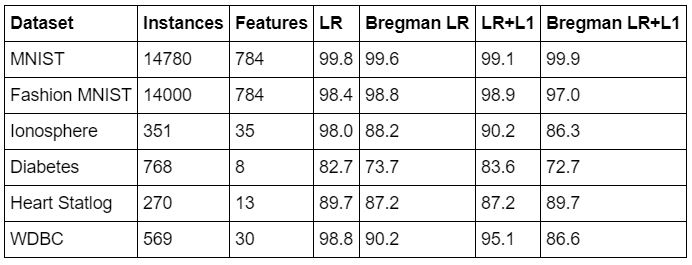
\includegraphics[scale=0.8]{./results.jpg}
 % results.jpg: 0x0 pixel, 0dpi, nanxnan cm, bb=
\end{center}


%% Bibliography %%
\begin{thebibliography}{10}

    \bibitem{logodds}
   {\sc  A.~Banerjee}
    \newblock 'An Analysis of Logistic Models:
Exponential Family Connections and Online Performance'.
    \newblock {\em 2007 SIAM International Conference on Data Mining}
    2007.  
    

    

    \bibitem{mean}
    {\sc A.~Banerjee, X.~Gou, H.~Wang}
    \newblock  'On the Optimality of Conditional Expectation as a Bregman Predictor'
    \newblock {\em IEEE Trans. on Information Theory} Vol 51(7)
    2005.  
    
    \bibitem{Bi}
{\sc J.~ Borwein and A.~ Lewis}, {\em Convex Analysis and Nonlinear Optimization}, (2 ed.). Springer. p. 76, 2006.

\bibitem{Collins}
   {\sc  M.~Collins, R.E.~Schapire, Y.~Singer}
    \newblock 'Logistic Regression, AdaBoost and Bregman Distances'
    \newblock {\em Machine Learning}, 48(1/2/3).
    2002.
    

    \bibitem{pietra}
    {\sc S.~Della Pietra, V.~Della Pietra, J.~Lafferty}, 'Duality and Auxiliary Functions for Bregman Distances', {\em Tech. rep. CMU-CS-01-109, School of Computer Science, Carnegie Mellon University.} 2001.
    
\bibitem{GLM}
{\sc A.~J.~ Dobson and A.~G.~ Barnett}, {\em Introduction to Generalized Linear Models},  Boca Raton, FL: Chapman and Hall/CRC, 2008.


    \bibitem{Someone2000}
   {\sc  T.~Huang, M.~Gupta}
    \newblock Bregman distance to L1 regularized logistic regression.
    \newblock {\em International Conference on Pattern Recognition}
    2008.  
    

\bibitem{NEF}
{\sc C.~ Morris}, "Natural Exponential Families with Quadratic Variance Functions", Annals of Statistics,
10 (1), p65-80. 1982

\bibitem{flash}
{\sc F.~ Nielsen, V.~ Garcia}, "Statistical exponential families: A digest with flash cards", arXiv:0911.4863v2, 2011.

\bibitem{Cheng}
{\sc R.~ Nock, A.~ Menon and C.~ Ong}, "A scaled Bregman theorem with applications", NIPS'16 Proceedings of the 30th International Conference on Neural Information Processing Systems, p. 19-27, 2016. 




\end{thebibliography}


\end{document}

